%%%%%%%%%%%%%%%%%%%%%%%%%%%%%%%%%%%%%%%%%
% Beamer Presentation
% LaTeX Template
% Version 1.0 (10/11/12)
%
% This template has been downloaded from:
% http://www.LaTeXTemplates.com
%
% License:
% CC BY-NC-SA 3.0 (http://creativecommons.org/licenses/by-nc-sa/3.0/)
%
%%%%%%%%%%%%%%%%%%%%%%%%%%%%%%%%%%%%%%%%%

%----------------------------------------------------------------------------------------
%	PACKAGES AND THEMES
%----------------------------------------------------------------------------------------

\documentclass{beamer}

\mode<presentation> {

% The Beamer class comes with a number of default slide themes
% which change the colors and layouts of slides. Below this is a list
% of all the themes, uncomment each in turn to see what they look like.

\usetheme{default}
%\usetheme{AnnArbor}
%\usetheme{Antibes}
%\usetheme{Bergen}
%\usetheme{Berkeley}
%\usetheme{Berlin}
%\usetheme{Boadilla}
%\usetheme{CambridgeUS}
%\usetheme{Copenhagen}
%\usetheme{Darmstadt}
%\usetheme{Dresden}
%\usetheme{Frankfurt}
%\usetheme{Goettingen}
%\usetheme{Hannover}
%\usetheme{Ilmenau}
%\usetheme{JuanLesPins}
%\usetheme{Luebeck}
%\usetheme{Madrid}
%\usetheme{Malmoe}
%\usetheme{Marburg}
%\usetheme{Montpellier}
%\usetheme{PaloAlto}
%\usetheme{Pittsburgh}
%\usetheme{Rochester}
%\usetheme{Singapore}
%\usetheme{Szeged}
%\usetheme{Warsaw}

% As well as themes, the Beamer class has a number of color themes
% for any slide theme. Uncomment each of these in turn to see how it
% changes the colors of your current slide theme.

%\usecolortheme{albatross}
%\usecolortheme{beaver}
%\usecolortheme{beetle}
%\usecolortheme{crane}
%\usecolortheme{dolphin}
%\usecolortheme{dove}
%\usecolortheme{fly}
%\usecolortheme{lily}
%\usecolortheme{orchid}
%\usecolortheme{rose}
%\usecolortheme{seagull}
%\usecolortheme{seahorse}
%\usecolortheme{whale}
%\usecolortheme{wolverine}

%\setbeamertemplate{footline} % To remove the footer line in all slides uncomment this line
\setbeamertemplate{footline}[page number] % To replace the footer line in all slides with a simple slide count uncomment this line

\setbeamertemplate{navigation symbols}{} % To remove the navigation symbols from the bottom of all slides uncomment this line
}
\newenvironment{changemargin}[2]{%
\begin{list}{}{%
\setlength{\topsep}{0pt}%
\setlength{\leftmargin}{#1}%
\setlength{\rightmargin}{#2}%
\setlength{\listparindent}{\parindent}%
\setlength{\itemindent}{\parindent}%
\setlength{\parsep}{\parskip}%
}%
\item[]}{\end{list}}
%\usepackage[greek,german]{babel}
\usepackage{graphicx} % Allows including images
\usepackage{booktabs} % Allows the use of \toprule, \midrule and \bottomrule in tables
\usepackage{amsmath}
\usepackage{slashed}
\usepackage{color}
\usepackage{rotating}
%----------------------------------------------------------------------------------------
%	TITLE PAGE
%----------------------------------------------------------------------------------------

\title{LFV analysis status report} % The short title appears at the bottom of every slide, the full title is only on the title page

\author{\underline{Author} \and Author} % Your name

\author{S.~Banerjee, D.~Biswas and \textbf{\underline{A.~Pathak}}}


\institute{\begin{minipage}{0.5\textwidth}\centering
\includegraphics[scale=0.1]{/afs/cern.ch/user/s/swaban/public/university-of-louisville-logo.png}
\end{minipage}}
\date{{LFV meeting}\\\today\\} % Date, can be changed to a custom date


\begin{document}

\begin{frame}
\titlepage % Print the title page as the first slide
\end{frame}
%%-----------------------------------------------
%\begin{frame}
%\frametitle{Fit value for Jet\_jes }
%\vspace*{-0.05cm}
%\begin{table}
%{\scalebox{.62}{
%\begin{tabular}{| l | c | c | c |c | c |}\hline\hline
%
%& H $\to$ \boldmath$ { \mu\tau_{had}}$ & H $\to$ \boldmath$ { \mu\tau_{had}}$ & H $\to$ \boldmath$ { \mu\tau_{had}}$& H $\to$ \boldmath$ { \mu\tau_{had}}$ & H $\to$ \boldmath$ { \mu\tau_{had}}$ \\
%& (Non-VBF) & (VBF) & (Comb) & (VBF decorr) & (Comb decorr) \\\hline
%jet\_jes\_bjes\_response & &-0.03 \boldmath${^{ 0.98}_{-0.99}}$&0.10 \boldmath${^{ 1.08}_{-0.97}}$&&\\\hline
%jet\_jes\_effectivenp\_1&-0.70 \boldmath${^{ 1.01}_{-0.75}}$ &0.09 \boldmath${^{ 1.05}_{-1.07}}$ &-0.58 \boldmath${^{ 1.04}_{-0.73}}$ &0.01 \boldmath${^{ 1.00}_{-0.98}}$ &-0.70 \boldmath${^{ 0.98}_{-0.74}}$ \\\hline
%jet\_jes\_effectivenp\_2&-0.12 \boldmath${^{ 0.95}_{-0.97}}$ & 0.03 \boldmath${^{ 0.95}_{-0.95}}$&-0.17 \boldmath${^{ 1.17}_{-0.87}}$ & 0.00 \boldmath${^{ 1.00}_{-1.00}}$&-0.14 \boldmath${^{ 0.95}_{-0.96}}$ \\\hline
%jet\_jes\_effectivenp\_3&-0.39 \boldmath${^{ 0.94}_{-0.96}}$ & 0.20 \boldmath${^{ 0.95}_{-0.97}}$& -0.20 \boldmath${^{ 0.98}_{-0.93}}$& &-0.41 \boldmath${^{ 0.93}_{-0.96}}$ \\\hline
%jet\_jes\_effectivenp\_4& -0.01 \boldmath${^{ 0.99}_{-0.99}}$& 0.04 \boldmath${^{ 0.95}_{-0.97}}$& -0.08 \boldmath${^{ 1.27}_{-0.90}}$& &-0.02 \boldmath${^{ 0.99}_{-0.99}}$ \\\hline
%jet\_jes\_effectivenp\_5&-0.04 \boldmath${^{ 1.02}_{-1.01}}$ &-0.10 \boldmath${^{ 0.95}_{-0.96}}$ & -0.11 \boldmath${^{ 0.96}_{-1.29}}$& &-0.05 \boldmath${^{ 1.02}_{-1.01}}$ \\\hline
%jet\_jes\_effectivenp\_6& 0.01 \boldmath${^{ 0.97}_{-0.97}}$& -0.09 \boldmath${^{ 0.90}_{-0.93}}$& -0.10 \boldmath${^{ 0.81}_{-0.96}}$& &0.01 \boldmath${^{ 0.97}_{-0.97}}$ \\\hline
%jet\_jes\_effectivenp\_7& 0.06 \boldmath${^{ 1.00}_{-0.99}}$& 0.40 \boldmath${^{ 0.92}_{-0.89}}$& 0.51 \boldmath${^{ 0.92}_{-1.24}}$& &0.08 \boldmath${^{ 0.99}_{-0.99}}$ \\\hline
%jet\_jes\_effectivenp\_8restterm& -0.04 \boldmath${^{ 1.03}_{-1.02}}$& 0.11 \boldmath${^{ 0.98}_{-0.96}}$& 0.22 \boldmath${^{ 0.98}_{-1.29}}$& 0.00 \boldmath${^{ 1.00}_{-1.00}}$&-0.05 \boldmath${^{ 1.03}_{-1.02}}$ \\\hline
%jet\_jes\_etaintercalibration\_modelling& 0.27 \boldmath${^{ 0.97}_{-1.20}}$& 0.14 \boldmath${^{ 0.99}_{-0.96}}$& 0.47 \boldmath${^{ 0.87}_{-1.09}}$& 0.01 \boldmath${^{ 0.99}_{-0.98}}$&0.31 \boldmath${^{ 0.95}_{-1.19}}$ \\\hline
%jet\_jes\_etaintercalibration\_nonclosure& 0.56 \boldmath${^{ 0.73}_{-1.34}}$& 0.06 \boldmath${^{ 0.97}_{-0.97}}$& 0.54 \boldmath${^{ 0.73}_{-1.20}}$&0.00 \boldmath${^{ 1.00}_{-1.00}}$ &0.54 \boldmath${^{ 0.73}_{-1.34}}$ \\\hline
%jet\_jes\_etaintercalibration\_totalstat&-0.03 \boldmath${^{ 0.89}_{-0.91}}$ & -0.25 \boldmath${^{ 0.95}_{-0.96}}$& -0.22 \boldmath${^{ 0.81}_{-0.97}}$&0.00 \boldmath${^{ 1.00}_{-1.00}}$ &-0.03 \boldmath${^{ 0.89}_{-0.90}}$ \\\hline
%jet\_jes\_flavor\_composition& 0.21 \boldmath${^{ 0.72}_{-0.78}}$& 0.19 \boldmath${^{ 0.93}_{-0.91}}$& 0.14 \boldmath${^{ 0.68}_{-0.72}}$& 0.00 \boldmath${^{ 1.00}_{-1.00}}$&0.23 \boldmath${^{ 0.69}_{-0.74}}$ \\\hline
%jet\_jes\_flavor\_response& -0.26 \boldmath${^{ 0.94}_{-0.96}}$& -0.17 \boldmath${^{ 0.89}_{-0.94}}$& -0.37 \boldmath${^{ 0.92}_{-1.06}}$& -0.01 \boldmath${^{ 0.99}_{-0.99}}$& -0.30 \boldmath${^{ 0.94}_{-0.95}}$\\\hline
%jet\_jes\_pileup\_offsetmu& -0.15 \boldmath${^{ 0.72}_{-0.82}}$& -0.09 \boldmath${^{ 0.89}_{-0.94}}$& -0.20 \boldmath${^{ 0.64}_{-0.79}}$& -0.00 \boldmath${^{ 0.99}_{-1.00}}$&-0.18 \boldmath${^{ 0.70}_{-0.82}}$ \\\hline
%jet\_jes\_pileup\_offsetnpv& 0.02 \boldmath${^{ 0.67}_{-0.67}}$& 0.04 \boldmath${^{ 0.98}_{-0.97}}$&0.09 \boldmath${^{ 0.68}_{-0.63}}$ &0.01 \boldmath${^{ 1.00}_{-0.99}}$ &0.01 \boldmath${^{ 0.67}_{-0.67}}$ \\\hline
%jet\_jes\_pileup\_ptterm& 0.53 \boldmath${^{ 0.94}_{-0.94}}$& 0.17 \boldmath${^{ 1.00}_{-1.09}}$&  0.70 \boldmath${^{ 0.90}_{-1.08}}$&0.00 \boldmath${^{ 1.00}_{-1.00}}$ &0.56 \boldmath${^{ 0.93}_{-0.94}}$ \\\hline
%jet\_jes\_pileup\_rhotopology& -0.40 \boldmath${^{ 0.99}_{-0.93}}$& 0.30 \boldmath${^{ 0.90}_{-1.20}}$& -0.30 \boldmath${^{ 0.97}_{-0.92}}$&0.01 \boldmath${^{ 0.99}_{-0.98}}$ &-0.35 \boldmath${^{ 0.97}_{-0.92}}$ \\\hline
%jet\_jes\_punchthrough\_mc15& & -0.06 \boldmath${^{ 0.95}_{-0.93}}$& -0.17 \boldmath${^{ 1.24}_{-0.95}}$& & \\ \hline
%jet\_jes\_singleparticle\_highpt& & -0.03 \boldmath${^{ 0.98}_{-0.99}}$& 0.10 \boldmath${^{ 1.08}_{-0.97}}$& & \\ \hline
%
%
%\end{tabular}
%}}
%\end{table}
%\end{frame}
%-----------------------------------------------
\begin{frame}
\frametitle{Fit value for Jet\_jes [before decorralation]}
\vspace*{-0.05cm}
\begin{table}
{\scalebox{.55}{
\begin{tabular}{| l | c | c | c| c | c |}\hline\hline

                                         & H $\to$ \boldmath$ { \mu\tau_{had}}$   & H $\to$ \boldmath$ { \mu\tau_{had}}$   & H $\to$ \boldmath$ { \mu\tau_{had}}$   \\
                                         & (Non-VBF)                              & (VBF)                                 & (Comb)                               \\ \hline
jet\_jes\_bjes\_response                 &                                        & -0.03 \boldmath${^{ 0.98}_{-0.99}}$     &  0.10 \boldmath${^{ 1.08}_{-0.97}}$     \\ \hline
jet\_jes\_effectivenp\_1                 & -0.70 \boldmath${^{ 1.01}_{-0.75}}$      &  0.09 \boldmath${^{ 1.05}_{-1.07}}$     & -0.58 \boldmath${^{ 1.04}_{-0.73}}$      \\ \hline
jet\_jes\_effectivenp\_2                 & -0.12 \boldmath${^{ 0.95}_{-0.97}}$      &  0.03 \boldmath${^{ 0.95}_{-0.95}}$     & \textcolor{red}{ -0.17 \boldmath${^{ 1.17}_{-0.87}}$    }  \\ \hline
jet\_jes\_effectivenp\_3                 & -0.39 \boldmath${^{ 0.94}_{-0.96}}$      &  0.20 \boldmath${^{ 0.95}_{-0.97}}$     & -0.20 \boldmath${^{ 0.98}_{-0.93}}$     \\ \hline
jet\_jes\_effectivenp\_4                 & -0.01 \boldmath${^{ 0.99}_{-0.99}}$      &  0.04 \boldmath${^{ 0.95}_{-0.97}}$     & -0.08 \boldmath${^{ 1.27}_{-0.90}}$     \\ \hline
jet\_jes\_effectivenp\_5                 & -0.04 \boldmath${^{ 1.02}_{-1.01}}$      & -0.10 \boldmath${^{ 0.95}_{-0.96}}$     & -0.11 \boldmath${^{ 0.96}_{-1.29}}$     \\ \hline
jet\_jes\_effectivenp\_6                 &  0.01 \boldmath${^{ 0.97}_{-0.97}}$      & -0.09 \boldmath${^{ 0.90}_{-0.93}}$     & -0.10 \boldmath${^{ 0.81}_{-0.96}}$     \\ \hline
jet\_jes\_effectivenp\_7                 &  0.06 \boldmath${^{ 1.00}_{-0.99}}$      &  0.40 \boldmath${^{ 0.92}_{-0.89}}$     &  0.51 \boldmath${^{ 0.92}_{-1.24}}$     \\ \hline
jet\_jes\_effectivenp\_8restterm         & -0.04 \boldmath${^{ 1.03}_{-1.02}}$      &  0.11 \boldmath${^{ 0.98}_{-0.96}}$     &  \textcolor{red}{ 0.22 \boldmath${^{ 0.98}_{-1.29}}$    }  \\ \hline
jet\_jes\_etaintercalibration\_modelling &  0.27 \boldmath${^{ 0.97}_{-1.20}}$      &  0.14 \boldmath${^{ 0.99}_{-0.96}}$     &  \textcolor{red}{ 0.47 \boldmath${^{ 0.87}_{-1.09}}$    } \\ \hline
jet\_jes\_etaintercalibration\_nonclosure&  0.56 \boldmath${^{ 0.73}_{-1.34}}$      &  0.06 \boldmath${^{ 0.97}_{-0.97}}$     &  0.54 \boldmath${^{ 0.73}_{-1.20}}$     \\ \hline
jet\_jes\_etaintercalibration\_totalstat & -0.03 \boldmath${^{ 0.89}_{-0.91}}$      & -0.25 \boldmath${^{ 0.95}_{-0.96}}$     & -0.22 \boldmath${^{ 0.81}_{-0.97}}$     \\ \hline
jet\_jes\_flavor\_composition            &  0.21 \boldmath${^{ 0.72}_{-0.78}}$      &  0.19 \boldmath${^{ 0.93}_{-0.91}}$     & \textcolor{red}{  0.14 \boldmath${^{ 0.68}_{-0.72}}$    } \\ \hline
jet\_jes\_flavor\_response               & -0.26 \boldmath${^{ 0.94}_{-0.96}}$      & -0.17 \boldmath${^{ 0.89}_{-0.94}}$     & \textcolor{red}{ -0.37 \boldmath${^{ 0.92}_{-1.06}}$    } \\ \hline
jet\_jes\_pileup\_offsetmu               & -0.15 \boldmath${^{ 0.72}_{-0.82}}$      & -0.09 \boldmath${^{ 0.89}_{-0.94}}$     & \textcolor{red}{ -0.20 \boldmath${^{ 0.64}_{-0.79}}$    } \\ \hline
jet\_jes\_pileup\_offsetnpv              &  0.02 \boldmath${^{ 0.67}_{-0.67}}$      &  0.04 \boldmath${^{ 0.98}_{-0.97}}$     & \textcolor{red}{ 0.09 \boldmath${^{ 0.68}_{-0.63}}$    } \\ \hline
jet\_jes\_pileup\_ptterm                 &  0.53 \boldmath${^{ 0.94}_{-0.94}}$      &  0.17 \boldmath${^{ 1.00}_{-1.09}}$     & \textcolor{red}{ 0.70 \boldmath${^{ 0.90}_{-1.08}}$    } \\ \hline
jet\_jes\_pileup\_rhotopology            & -0.40 \boldmath${^{ 0.99}_{-0.93}}$      &  0.30 \boldmath${^{ 0.90}_{-1.20}}$     & -0.30 \boldmath${^{ 0.97}_{-0.92}}$     \\ \hline
jet\_jes\_punchthrough\_mc15             &                                        & -0.06 \boldmath${^{ 0.95}_{-0.93}}$     & -0.17 \boldmath${^{ 1.24}_{-0.95}}$   \\ \hline
jet\_jes\_singleparticle\_highpt         &                                        & -0.03 \boldmath${^{ 0.98}_{-0.99}}$     &  0.10 \boldmath${^{ 1.08}_{-0.97}}$   \\ \hline

\end{tabular}
}}
\end{table}

Some nuisance parameters for combination were outside the range set by non-vbf and vbf.

\end{frame}
%-----------------------------------------------
\begin{frame}
\frametitle{Fit value for Jet\_jes [after decorralation]}
\vspace*{-0.05cm}
\begin{table}
{\scalebox{.55}{
\begin{tabular}{| l | c | c | c|}\hline\hline

                                         & H $\to$ \boldmath$ { \mu\tau_{had}}$    & H $\to$ \boldmath$ { \mu\tau_{had}}$  & H $\to$ \boldmath$ { \mu\tau_{had}}$    \\
                                         & (Non-VBF)                              & (VBF decorr)                          & (Comb decorr)                          \\ \hline
jet\_jes\_bjes\_response                 &                                        &                                       &                                        \\ \hline
jet\_jes\_effectivenp\_1                 & -0.70 \boldmath${^{ 1.01}_{-0.75}}$      &  0.01 \boldmath${^{ 1.00}_{-0.98}}$     & -0.70 \boldmath${^{ 0.98}_{-0.74}}$      \\ \hline
jet\_jes\_effectivenp\_2                 & -0.12 \boldmath${^{ 0.95}_{-0.97}}$      &  0.00 \boldmath${^{ 1.00}_{-1.00}}$     & -0.14 \boldmath${^{ 0.95}_{-0.96}}$      \\ \hline
jet\_jes\_effectivenp\_3                 & -0.39 \boldmath${^{ 0.94}_{-0.96}}$      &                                       & -0.41 \boldmath${^{ 0.93}_{-0.96}}$      \\ \hline
jet\_jes\_effectivenp\_4                 & -0.01 \boldmath${^{ 0.99}_{-0.99}}$      &                                       & -0.02 \boldmath${^{ 0.99}_{-0.99}}$      \\ \hline
jet\_jes\_effectivenp\_5                 & -0.04 \boldmath${^{ 1.02}_{-1.01}}$      &                                       & -0.05 \boldmath${^{ 1.02}_{-1.01}}$      \\ \hline
jet\_jes\_effectivenp\_6                 &  0.01 \boldmath${^{ 0.97}_{-0.97}}$      &                                       &  0.01 \boldmath${^{ 0.97}_{-0.97}}$      \\ \hline
jet\_jes\_effectivenp\_7                 &  0.06 \boldmath${^{ 1.00}_{-0.99}}$      &                                       &  0.08 \boldmath${^{ 0.99}_{-0.99}}$      \\ \hline
jet\_jes\_effectivenp\_8restterm         & -0.04 \boldmath${^{ 1.03}_{-1.02}}$      &  0.00 \boldmath${^{ 1.00}_{-1.00}}$     & -0.05 \boldmath${^{ 1.03}_{-1.02}}$      \\ \hline
jet\_jes\_etaintercalibration\_modelling &  0.27 \boldmath${^{ 0.97}_{-1.20}}$      &  0.01 \boldmath${^{ 0.99}_{-0.98}}$   &  0.31 \boldmath${^{ 0.95}_{-1.19}}$      \\ \hline
jet\_jes\_etaintercalibration\_nonclosure&  0.56 \boldmath${^{ 0.73}_{-1.34}}$      &  0.00 \boldmath${^{ 1.00}_{-1.00}}$   &  0.54 \boldmath${^{ 0.73}_{-1.34}}$      \\ \hline
jet\_jes\_etaintercalibration\_totalstat & -0.03 \boldmath${^{ 0.89}_{-0.91}}$      &  0.00 \boldmath${^{ 1.00}_{-1.00}}$   & -0.03 \boldmath${^{ 0.89}_{-0.90}}$      \\ \hline
jet\_jes\_flavor\_composition            &  0.21 \boldmath${^{ 0.72}_{-0.78}}$      &  0.00 \boldmath${^{ 1.00}_{-1.00}}$   &  0.23 \boldmath${^{ 0.69}_{-0.74}}$      \\ \hline
jet\_jes\_flavor\_response               & -0.26 \boldmath${^{ 0.94}_{-0.96}}$      & -0.01 \boldmath${^{ 0.99}_{-0.99}}$   & -0.30 \boldmath${^{ 0.94}_{-0.95}}$      \\ \hline
jet\_jes\_pileup\_offsetmu               & -0.15 \boldmath${^{ 0.72}_{-0.82}}$      & -0.00 \boldmath${^{ 0.99}_{-1.00}}$   & -0.18 \boldmath${^{ 0.70}_{-0.82}}$      \\ \hline
jet\_jes\_pileup\_offsetnpv              &  0.02 \boldmath${^{ 0.67}_{-0.67}}$      &  0.01 \boldmath${^{ 1.00}_{-0.99}}$   &  0.01 \boldmath${^{ 0.67}_{-0.67}}$      \\ \hline
jet\_jes\_pileup\_ptterm                 &  0.53 \boldmath${^{ 0.94}_{-0.94}}$      &  0.00 \boldmath${^{ 1.00}_{-1.00}}$   &  0.56 \boldmath${^{ 0.93}_{-0.94}}$      \\ \hline
jet\_jes\_pileup\_rhotopology            & -0.40 \boldmath${^{ 0.99}_{-0.93}}$      &  0.01 \boldmath${^{ 0.99}_{-0.98}}$   & -0.35 \boldmath${^{ 0.97}_{-0.92}}$      \\ \hline
jet\_jes\_punchthrough\_mc15             &                                        &                                       &                                        \\ \hline
jet\_jes\_singleparticle\_highpt         &                                        &                                       &                                        \\ \hline

\end{tabular}
}}
\end{table}

\begin{itemize}
  \item fitted values in VBF\_decorr channel are close to zero (no bias)
  \item comb\_decorr is close to non-vbf (no hidden correlations)
 \end{itemize}

\end{frame}
%-----------------------------------------------
\begin{frame}
\frametitle{Fit value for Jet\_jes [after decorralation]}
\vspace*{-0.05cm}
\begin{table}
{\scalebox{.55}{
\begin{tabular}{| l |c | c |}\hline\hline

& H $\to$ \boldmath$ { \mu\tau_{had}}$ & H $\to$ \boldmath$ { \mu\tau_{had}}$ \\
& (VBF decorr) & (Comb decorr) \\\hline
jet\_jes\_bjes\_response\_vbf &-0.02 \boldmath${^{ 0.98}_{-0.99}}$ & 0.10 \boldmath${^{ 0.95}_{-0.95}}$ \\\hline
jet\_jes\_effectivenp\_1\_vbf & 0.09 \boldmath${^{ 1.04}_{-1.07}}$ & 0.13 \boldmath${^{ 1.02}_{-1.06}}$ \\\hline
jet\_jes\_effectivenp\_2\_vbf & 0.03 \boldmath${^{ 0.95}_{-0.95}}$ & 0.08 \boldmath${^{ 0.92}_{-0.91}}$ \\\hline
jet\_jes\_effectivenp\_3\_vbf & 0.20 \boldmath${^{ 0.95}_{-0.97}}$ & 0.16 \boldmath${^{ 0.92}_{-0.94}}$ \\\hline
jet\_jes\_effectivenp\_4\_vbf & 0.05 \boldmath${^{ 0.95}_{-0.97}}$ & 0.13 \boldmath${^{ 0.93}_{-0.93}}$ \\\hline
jet\_jes\_effectivenp\_5\_vbf &-0.10 \boldmath${^{ 0.95}_{-0.96}}$ &-0.21 \boldmath${^{ 0.97}_{-0.96}}$ \\\hline
jet\_jes\_effectivenp\_6\_vbf                 &-0.08 \boldmath${^{ 0.90}_{-0.93}}$ &-0.16 \boldmath${^{ 0.85}_{-0.91}}$ \\\hline
jet\_jes\_effectivenp\_7\_vbf                 & 0.40 \boldmath${^{ 0.92}_{-0.89}}$ & 0.39 \boldmath${^{ 0.92}_{-0.88}}$ \\\hline
jet\_jes\_effectivenp\_8restterm\_vbf         & 0.12 \boldmath${^{ 0.98}_{-0.96}}$ & 0.08 \boldmath${^{ 0.97}_{-0.95}}$ \\\hline
jet\_jes\_etaintercalibration\_modelling\_vbf & 0.13 \boldmath${^{ 0.98}_{-0.96}}$ & 0.13 \boldmath${^{ 0.97}_{-0.93}}$ \\\hline
jet\_jes\_etaintercalibration\_nonclosure\_vbf& 0.05 \boldmath${^{ 0.97}_{-0.97}}$ & 0.07 \boldmath${^{ 0.96}_{-0.96}}$ \\\hline
jet\_jes\_etaintercalibration\_totalstat\_vbf &-0.24 \boldmath${^{ 0.95}_{-0.96}}$ &-0.23 \boldmath${^{ 0.93}_{-0.96}}$ \\\hline
jet\_jes\_flavor\_composition\_vbf            & 0.18 \boldmath${^{ 0.93}_{-0.90}}$ & 0.19 \boldmath${^{ 0.93}_{-0.91}}$ \\\hline
jet\_jes\_flavor\_response\_vbf               &-0.17 \boldmath${^{ 0.89}_{-0.94}}$ &-0.15 \boldmath${^{ 0.88}_{-0.94}}$ \\\hline
jet\_jes\_pileup\_offsetmu\_vbf               &-0.10 \boldmath${^{ 0.90}_{-0.94}}$ &-0.07 \boldmath${^{ 0.86}_{-0.90}}$ \\\hline
jet\_jes\_pileup\_offsetnpv\_vbf              & 0.04 \boldmath${^{ 0.98}_{-0.97}}$ & 0.05 \boldmath${^{ 0.98}_{-0.97}}$ \\\hline
jet\_jes\_pileup\_ptterm\_vbf                 & 0.16 \boldmath${^{ 1.00}_{-1.09}}$ & 0.12 \boldmath${^{ 1.01}_{-1.06}}$\\\hline
jet\_jes\_pileup\_rhotopology\_vbf            & 0.30 \boldmath${^{ 0.90}_{-1.21}}$ & 0.28 \boldmath${^{ 0.89}_{-1.11}}$ \\\hline
jet\_jes\_punchthrough\_mc15\_vbf             &-0.06 \boldmath${^{ 0.95}_{-0.93}}$ &-0.10 \boldmath${^{ 0.92}_{-0.92}}$ \\\hline
jet\_jes\_singleparticle\_highpt\_vbf         &-0.02 \boldmath${^{ 0.98}_{-0.99}}$ & 0.10 \boldmath${^{ 0.95}_{-0.95}}$\\\hline

\end{tabular}
}}
\end{table}

These newly created nuisance parameters do NOT change much when fitted only in VBF\_decorr channel or in combination\_decorr channel.
This means that they DO NOT pick up any new un-intended correlation from other nuisance parameters.

\end{frame}
%-----------------------------------------------
\begin{frame}
\frametitle{POI Results for MVA}
\begin{normalsize}

  \begin{center}
    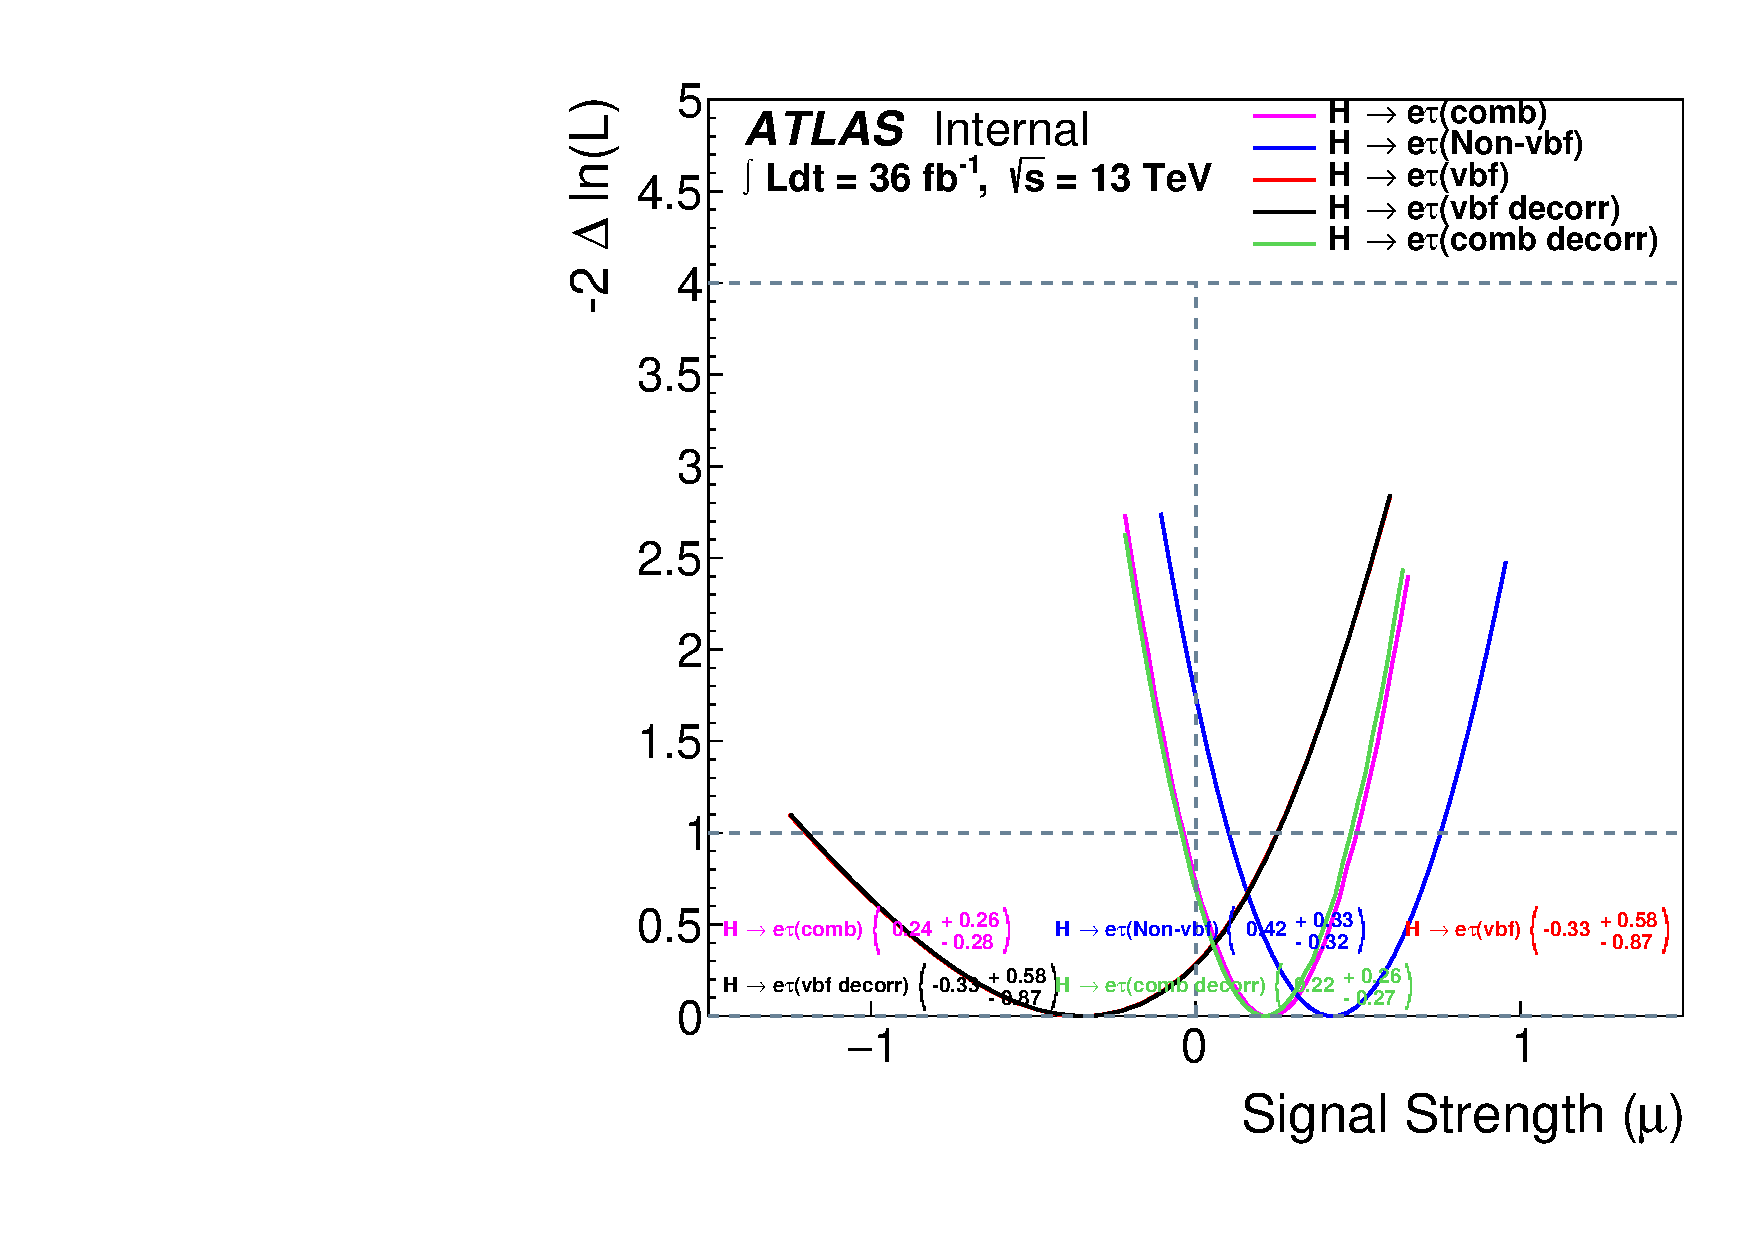
\includegraphics[height=.7\textheight,type=png,ext=.png,read=.png]{/afs/cern.ch/user/a/atpathak/afswork/public/Pixel/LFV_Plots/NPscans_figures/SigXsecOverSM_ObsData_lfv_125}
   \end{center}

  \vspace*{-0.5cm}
  \begin{table}
{\scalebox{.65}{
\begin{tabular}{| l | c | c | c |c | c |}\hline\hline
& H $\to$ \boldmath$ { \mu\tau_{had}}$ & H $\to$ \boldmath$ { \mu\tau_{had}}$ & H $\to$ \boldmath$ { \mu\tau_{had}}$& H $\to$ \boldmath$ { \mu\tau_{had}}$ & H $\to$ \boldmath$ { \mu\tau_{had}}$ \\
& (Non-VBF) & (VBF) & (Comb) & (VBF decorr) & (Comb decorr) \\\hline
SigXsecOverSM & -0.21 \boldmath${^{ 0.31}_{-0.32}}$ & -0.08 \boldmath${^{ 0.58}_{-0.83}}$ & \textcolor{magenta}{-0.07 \boldmath${^{ 0.23}_{-0.23}}$}&-0.09 \boldmath${^{+0.58}_{-0.84}}$ &\textcolor{green}{-0.15 \boldmath${^{ 0.27}_{-0.26}}$} \\\hline
\end{tabular}
}}
\end{table}
\end{normalsize}
\end{frame}
%-----------------------------------------------
\begin{frame}
\frametitle{Summary}
\begin{scriptsize}
\vspace*{0.2cm}
\begin{itemize}
\item The previously fitted value of POI (mu) for a combination of mutauhad (-0.07) was outside the range given by fitted values for mutauhad\_nonvbf (-0.21) and mutauhad\_vbf (-0.08).

\item We scanned 50 points between -1.5 and 1.5, that's why we got -.08 instead of -0.09, mentioned in the paper; but it is close enough.

\item The VBF channel has 1 Signal region and 1 control region (Ztt, leplep).
We took the jet\_jes related nuisance parameters in VBF channel and changed their names.
Thus we obtained a VBF\_decorr channel where jet\_jes in the signal region have \_vbf appended to their names, while the jet\_jes in control region are kept untouched.

\item
We find that this VBF\_decorr has a muhat (-0.09) quite close to VBF channel (-0.08).
This shows that the decorrelation doesn't adversely affect the VBF channel.

\item
Then we make a new combination of non-VBF and VBF\_decorr and call it comb\_decorr.
The fitted muhat for this is -0.15 , eg. between -0.21 and -0.08.
This shows that the decorrelation has the desired effect on naive expectation for a combination.

\end{itemize}
\end{scriptsize}
\end{frame}
%---------------------------------------------------
\end{document}
%---------------------------------------------------
\begin{frame}
\frametitle{Fit value for Jet\_jes }
\vspace*{-0.05cm}
\begin{table}
{\scalebox{.65}{
\begin{tabular}{| l | c | c | c |c | c |}\hline\hline

& H $\to$ \boldmath$ { \mu\tau_{had}}$ & H $\to$ \boldmath$ { \mu\tau_{had}}$ & H $\to$ \boldmath$ { \mu\tau_{had}}$& H $\to$ \boldmath$ { \mu\tau_{had}}$ & H $\to$ \boldmath$ { \mu\tau_{had}}$ \\
& (Non-VBF) & (VBF) & (Comb) & (VBF decorr) & (Comb decorr) \\\hline
SigXsecOverSM & -0.21 \boldmath${^{ 0.31}_{-0.32}}$ & -0.08 \boldmath${^{ 0.58}_{-0.83}}$ & \textcolor{red}{-0.07 \boldmath${^{ 0.23}_{-0.23}}$}&-0.09 \boldmath${^{+0.58}_{-0.84}}$ &\textcolor{green}{-0.15 \boldmath${^{ 0.27}_{-0.26}}$} \\\hline
jet\_jes\_bjes\_response & &-0.03 \boldmath${^{ 0.98}_{-0.99}}$&0.10 \boldmath${^{ 1.08}_{-0.97}}$&&\\\hline
jet\_jes\_bjes\_response\_vbf & & & &-0.02 \boldmath${^{ 0.98}_{-0.99}}$ &0.10 \boldmath${^{ 0.95}_{-0.95}}$ \\\hline
jet\_jes\_effectivenp\_1&-0.70 \boldmath${^{ 1.01}_{-0.75}}$ &0.09 \boldmath${^{ 1.05}_{-1.07}}$ &-0.58 \boldmath${^{ 1.04}_{-0.73}}$ &0.01 \boldmath${^{ 1.00}_{-0.98}}$ &-0.70 \boldmath${^{ 0.98}_{-0.74}}$ \\\hline
jet\_jes\_effectivenp\_1\_vbf& & & &0.09 \boldmath${^{ 1.04}_{-1.07}}$ &0.13 \boldmath${^{ 1.02}_{-1.06}}$ \\\hline
jet\_jes\_effectivenp\_2&-0.12 \boldmath${^{ 0.95}_{-0.97}}$ & 0.03 \boldmath${^{ 0.95}_{-0.95}}$&-0.17 \boldmath${^{ 1.17}_{-0.87}}$ & 0.00 \boldmath${^{ 1.00}_{-1.00}}$&-0.14 \boldmath${^{ 0.95}_{-0.96}}$ \\\hline
jet\_jes\_effectivenp\_2\_vbf& & & &0.03 \boldmath${^{ 0.95}_{-0.95}}$ &0.08 \boldmath${^{ 0.92}_{-0.91}}$ \\\hline
jet\_jes\_effectivenp\_3&-0.39 \boldmath${^{ 0.94}_{-0.96}}$ & 0.20 \boldmath${^{ 0.95}_{-0.97}}$& -0.20 \boldmath${^{ 0.98}_{-0.93}}$& &-0.41 \boldmath${^{ 0.93}_{-0.96}}$ \\\hline
jet\_jes\_effectivenp\_3\_vbf& & & &0.20 \boldmath${^{ 0.95}_{-0.97}}$ &0.16 \boldmath${^{ 0.92}_{-0.94}}$ \\\hline
jet\_jes\_effectivenp\_4& -0.01 \boldmath${^{ 0.99}_{-0.99}}$& 0.04 \boldmath${^{ 0.95}_{-0.97}}$& -0.08 \boldmath${^{ 1.27}_{-0.90}}$& &-0.02 \boldmath${^{ 0.99}_{-0.99}}$ \\\hline
jet\_jes\_effectivenp\_4\_vbf& & & & 0.05 \boldmath${^{ 0.95}_{-0.97}}$&0.13 \boldmath${^{ 0.93}_{-0.93}}$ \\\hline
jet\_jes\_effectivenp\_5&-0.04 \boldmath${^{ 1.02}_{-1.01}}$ &-0.10 \boldmath${^{ 0.95}_{-0.96}}$ & -0.11 \boldmath${^{ 0.96}_{-1.29}}$& &-0.05 \boldmath${^{ 1.02}_{-1.01}}$ \\\hline
jet\_jes\_effectivenp\_5\_vbf& & & &-0.10 \boldmath${^{ 0.95}_{-0.96}}$ &-0.21 \boldmath${^{ 0.97}_{-0.96}}$ \\\hline
jet\_jes\_effectivenp\_6& 0.01 \boldmath${^{ 0.97}_{-0.97}}$& -0.09 \boldmath${^{ 0.90}_{-0.93}}$& -0.10 \boldmath${^{ 0.81}_{-0.96}}$& &0.01 \boldmath${^{ 0.97}_{-0.97}}$ \\\hline
jet\_jes\_effectivenp\_6\_vbf& & & & -0.08 \boldmath${^{ 0.90}_{-0.93}}$&-0.16 \boldmath${^{ 0.85}_{-0.91}}$ \\\hline
jet\_jes\_effectivenp\_7& 0.06 \boldmath${^{ 1.00}_{-0.99}}$& 0.40 \boldmath${^{ 0.92}_{-0.89}}$& 0.51 \boldmath${^{ 0.92}_{-1.24}}$& &0.08 \boldmath${^{ 0.99}_{-0.99}}$ \\\hline
jet\_jes\_effectivenp\_7\_vbf& & & & 0.40 \boldmath${^{ 0.92}_{-0.89}}$&0.39 \boldmath${^{ 0.92}_{-0.88}}$ \\\hline
jet\_jes\_effectivenp\_8restterm& -0.04 \boldmath${^{ 1.03}_{-1.02}}$& 0.11 \boldmath${^{ 0.98}_{-0.96}}$& 0.22 \boldmath${^{ 0.98}_{-1.29}}$& 0.00 \boldmath${^{ 1.00}_{-1.00}}$&-0.05 \boldmath${^{ 1.03}_{-1.02}}$ \\\hline
jet\_jes\_effectivenp\_8restterm\_vbf& & & & 0.12 \boldmath${^{ 0.98}_{-0.96}}$&0.08 \boldmath${^{ 0.97}_{-0.95}}$ \\\hline
\end{tabular}
}}
\end{table}
\end{frame}
%-----------------------------------------------
\begin{frame}
\frametitle{Fit value for Jet\_jes}
\vspace*{-0.05cm}
\begin{table}
{\scalebox{.55}{
\begin{tabular}{| l | c | c | c |c | c |}\hline\hline

& H $\to$ \boldmath$ { \mu\tau_{had}}$ & H $\to$ \boldmath$ { \mu\tau_{had}}$ & H $\to$ \boldmath$ { \mu\tau_{had}}$& H $\to$ \boldmath$ { \mu\tau_{had}}$ & H $\to$ \boldmath$ { \mu\tau_{had}}$ \\
& (Non-VBF) & (VBF) & (Comb) & (VBF decorr) & (Comb decorr) \\\hline
jet\_jes\_etaintercalibration\_modelling& 0.27 \boldmath${^{ 0.97}_{-1.20}}$& 0.14 \boldmath${^{ 0.99}_{-0.96}}$& 0.47 \boldmath${^{ 0.87}_{-1.09}}$& 0.01 \boldmath${^{ 0.99}_{-0.98}}$&0.31 \boldmath${^{ 0.95}_{-1.19}}$ \\\hline
jet\_jes\_etaintercalibration\_modelling\_vbf& & & & 0.13 \boldmath${^{ 0.98}_{-0.96}}$&0.13 \boldmath${^{ 0.97}_{-0.93}}$ \\\hline
jet\_jes\_etaintercalibration\_nonclosure& 0.56 \boldmath${^{ 0.73}_{-1.34}}$& 0.06 \boldmath${^{ 0.97}_{-0.97}}$& 0.54 \boldmath${^{ 0.73}_{-1.20}}$&0.00 \boldmath${^{ 1.00}_{-1.00}}$ &0.54 \boldmath${^{ 0.73}_{-1.34}}$ \\\hline
jet\_jes\_etaintercalibration\_nonclosure\_vbf& & & & 0.05 \boldmath${^{ 0.97}_{-0.97}}$&0.07 \boldmath${^{ 0.96}_{-0.96}}$ \\\hline
jet\_jes\_etaintercalibration\_totalstat&-0.03 \boldmath${^{ 0.89}_{-0.91}}$ & -0.25 \boldmath${^{ 0.95}_{-0.96}}$& -0.22 \boldmath${^{ 0.81}_{-0.97}}$&0.00 \boldmath${^{ 1.00}_{-1.00}}$ &-0.03 \boldmath${^{ 0.89}_{-0.90}}$ \\\hline
jet\_jes\_etaintercalibration\_totalstat\_vbf& & & & -0.24 \boldmath${^{ 0.95}_{-0.96}}$&-0.23 \boldmath${^{ 0.93}_{-0.96}}$ \\\hline
jet\_jes\_flavor\_composition& 0.21 \boldmath${^{ 0.72}_{-0.78}}$& 0.19 \boldmath${^{ 0.93}_{-0.91}}$& 0.14 \boldmath${^{ 0.68}_{-0.72}}$& 0.00 \boldmath${^{ 1.00}_{-1.00}}$&0.23 \boldmath${^{ 0.69}_{-0.74}}$ \\\hline
jet\_jes\_flavor\_composition\_vbf& & & & 0.18 \boldmath${^{ 0.93}_{-0.90}}$&0.19 \boldmath${^{ 0.93}_{-0.91}}$ \\\hline
jet\_jes\_flavor\_response& -0.26 \boldmath${^{ 0.94}_{-0.96}}$& -0.17 \boldmath${^{ 0.89}_{-0.94}}$& -0.37 \boldmath${^{ 0.92}_{-1.06}}$& -0.01 \boldmath${^{ 0.99}_{-0.99}}$& -0.30 \boldmath${^{ 0.94}_{-0.95}}$\\\hline
jet\_jes\_flavor\_response\_vbf& & & &-0.17 \boldmath${^{ 0.89}_{-0.94}}$ &-0.15 \boldmath${^{ 0.88}_{-0.94}}$ \\\hline
jet\_jes\_pileup\_offsetmu& -0.15 \boldmath${^{ 0.72}_{-0.82}}$& -0.09 \boldmath${^{ 0.89}_{-0.94}}$& -0.20 \boldmath${^{ 0.64}_{-0.79}}$& -0.00 \boldmath${^{ 0.99}_{-1.00}}$&-0.18 \boldmath${^{ 0.70}_{-0.82}}$ \\\hline
jet\_jes\_pileup\_offsetmu\_vbf& & & & -0.10 \boldmath${^{ 0.90}_{-0.94}}$&-0.07 \boldmath${^{ 0.86}_{-0.90}}$ \\\hline
jet\_jes\_pileup\_offsetnpv& 0.02 \boldmath${^{ 0.67}_{-0.67}}$& 0.04 \boldmath${^{ 0.98}_{-0.97}}$&0.09 \boldmath${^{ 0.68}_{-0.63}}$ &0.01 \boldmath${^{ 1.00}_{-0.99}}$ &0.01 \boldmath${^{ 0.67}_{-0.67}}$ \\\hline
jet\_jes\_pileup\_offsetnpv\_vbf& & & & 0.04 \boldmath${^{ 0.98}_{-0.97}}$&0.05 \boldmath${^{ 0.98}_{-0.97}}$ \\\hline
jet\_jes\_pileup\_ptterm& 0.53 \boldmath${^{ 0.94}_{-0.94}}$& 0.17 \boldmath${^{ 1.00}_{-1.09}}$&  0.70 \boldmath${^{ 0.90}_{-1.08}}$&0.00 \boldmath${^{ 1.00}_{-1.00}}$ &0.56 \boldmath${^{ 0.93}_{-0.94}}$ \\\hline
jet\_jes\_pileup\_ptterm\_vbf& & & & 0.16 \boldmath${^{ 1.00}_{-1.09}}$& 0.12 \boldmath${^{ 1.01}_{-1.06}}$\\\hline
jet\_jes\_pileup\_rhotopology& -0.40 \boldmath${^{ 0.99}_{-0.93}}$& 0.30 \boldmath${^{ 0.90}_{-1.20}}$& -0.30 \boldmath${^{ 0.97}_{-0.92}}$&0.01 \boldmath${^{ 0.99}_{-0.98}}$ &-0.35 \boldmath${^{ 0.97}_{-0.92}}$ \\\hline
jet\_jes\_pileup\_rhotopology\_vbf& & & & 0.30 \boldmath${^{ 0.90}_{-1.21}}$&0.28 \boldmath${^{ 0.89}_{-1.11}}$ \\\hline
jet\_jes\_punchthrough\_mc15& & -0.06 \boldmath${^{ 0.95}_{-0.93}}$& -0.17 \boldmath${^{ 1.24}_{-0.95}}$& & \\ \hline
jet\_jes\_punchthrough\_mc15\_vbf& & & & -0.06 \boldmath${^{ 0.95}_{-0.93}}$&-0.10 \boldmath${^{ 0.92}_{-0.92}}$ \\\hline
jet\_jes\_singleparticle\_highpt& & -0.03 \boldmath${^{ 0.98}_{-0.99}}$& 0.10 \boldmath${^{ 1.08}_{-0.97}}$& & \\ \hline
jet\_jes\_singleparticle\_highpt\_vbf& & & &-0.02 \boldmath${^{ 0.98}_{-0.99}}$ & 0.10 \boldmath${^{ 0.95}_{-0.95}}$\\\hline

\end{tabular}
}}
\end{table}
\end{frame}
%---------------------------------------------------
\end{document}
%----------------------------------------------
